\section{Grafisk bruger interface}
\textit{Dette afsnit omhandler design, implementering og test af Graphical User Interface (GUI), til visualisering af de udførte aktiviteter. Først designes GUI til det specifikke formål ud fra dets kravspecifikationer, hvorefter denne kan implementeres. Afslutningsvist bliver GUI testet i forhold til opstillede krav.}
\subsection{Design}
GUI benyttes til at motivere børn til en mere aktiv hverdag. Dette gøres ud fra \secref{motivation_boern}, hvor det beskrives at børn motiveres gennem succesoplevelser. GUI designes dermed ud fra at alle børn har mulighed for at optjene mange point, da pointene vægtes ud fra intensiteten, tiden samt typen af aktivitet.

Data fra algoritmerne vedrørende aktiviteterne gang, løb og cykling sendes til MATLAB, som det ses på \figref{fig:GUI}. Fra algoritmen vedrørende gang og løb sendes der to resultater. Resultaterne består først af et id, hvormed det kan identificeres hvorvidt data kommer fra accelerometeret eller gyroskopet. Derudover er der en peakværdi og et resultat af varighed siden sidst detekterede peak. Peakets værdi informere om hvilken aktivitet varigheden bør tillægges. Er peakværdien mellem 100 og 1100 skal varigheden lægges i tidsvariablen for gang, og er den over 1100 skal den lægges over i tidsvariablen for løb. Algoritmen for gyroskopets data udføres i MATLAB, hvor der opsamles et 4 sekunders data i et array, hvorefter det udføres en fft. Viser denne at der cykles, vil der tillægges 4 sekunder til tidsvariablen for cykling. Fra algoritmen vedrørende pulssensoren sendes data i form af BPM, beregnet over tre peaks. \\
Ved gang og løb modtages varigheden som samples og skal dermed omregnes til tid i minutter. Herefter ligges tiden over i en tidsvariabel for den tilhørende aktivitet. Denne vises som værdi for den enkelte aktivitet, så det er muligt at se hvor længe barnet har været aktiv ved de forskellige aktiviteter.

Hver aktivitet belønnes forskelligt, da det er væsentligt at få børnene til at løbe og cykle mere, end at gå. Dermed multipliceres tiden for løb med tre, for cykling med to og for gang med en. Derudover belønnes barnet for intensiteten af aktiviteten. Ud fra \secref{subsub:ak_int} beregnes den afrundede makspulsen samt pulsen for aktiviteter med henholdsvis lav, moderat og høj intensitet. Makspulsen for et barn på 9-12 år er gennemsnitligt 210 og en lav intensitet ligger dermed under 147, moderat intensitet er mellem 147 og 168 og høj intensitet ligger over 168. Aktivitetens point multipliceres med to ved høj intensitet, multipliceres med halvanden ved moderat intensitet, og multipliceres ikke ved lav intensitet. Pointene visualiseres ud for den enkelte aktivitet, så barnet kan se hvor mange point de har opnået ved udførslen for den enkelte aktivitet igennem en hel dag. For at aktivere børnene hver dag, samles dagens point for alle aktiviteter udført i løbet af dagen. Pointene vises grafisk som en søjle hvormed barnet kan få et overblik over antallet af point fra de forskellige dage. Søjlen afspejler hvor mange point børnene har opnået samt hvor stor en del der er opnået ved henholdsvis gang, løb og cykling.  

\begin{figure}[H]
	\centering
	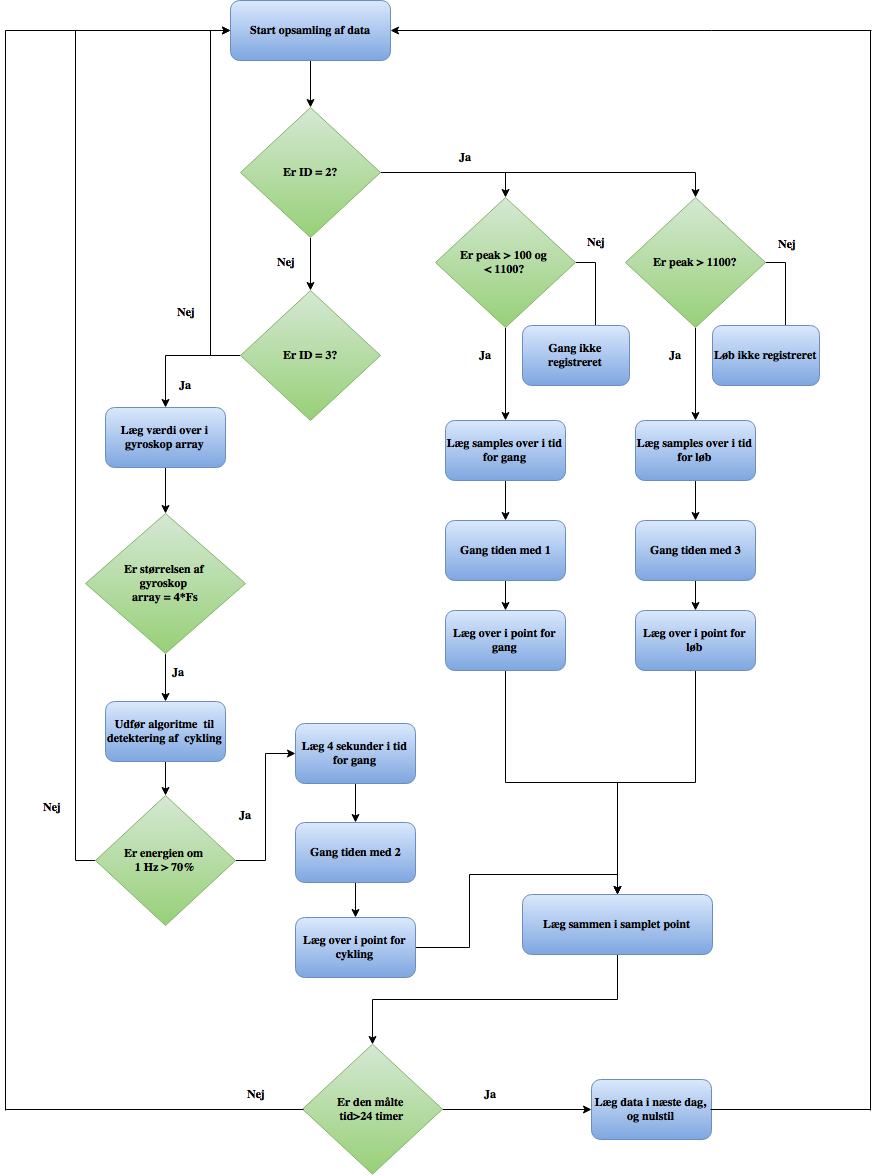
\includegraphics[scale=0.4]{figures/cDesign/pseudo_GUI.png}
	\caption{På figuren ses et flowchart som gennemgår hvorledes resultaterne fra de forskellige algoritmer behandles af GUI.}
	\label{fig:GUI}
\end{figure}

\subsection{Implementering}
GUI implementeres ved at anvende MATLABS funktion Graphical User Interface Design Environment (GUIDE). GUIDE er en funktion der gør det muligt at lave en specifik brugerflade med indbyggede funktioner.

Der indsættes en toggle button med teksten START, og når der trykkes på knappen, startes programmet, og teksten bliver ændret til STOP. Når programmet startes indhentes data fra mikrokontrolleren, som for accelerometeret kommer ind som [id, tid, peakværdi, puls]. Den første værdi er en repræsentation om dataen er fra gyroskopet eller fra accelerometeret. Den sidste værdi tredje værdi viderføres til løkker hvor det tjekkes hvorvidt det er et peak som repræsenteres af gang eller løb. Den anden værdi, som er en repræsentation af hvor mange samples der er mellem hvert peak, omregnes til minutter og lægges over i tidsvariablen for den pågældende aktivitet. Omregning udføres som \eqref{eq:tidsvariabel}. Derudover udføres en fft i MATL på gyroskopdata, når et array af fire sekunders data er fyldt. Ses der at fft'en er over 70 \% identisk, lægges 4 sekunder over i tidsvariabel for cykling. 
\begin{equation}
\label{eq:tidsvariabel}
	tidsvariabel = tid/samplingsfrekvens*0,016667
\end{equation}
Derudover skal tidsvariablen omregnes til point, ved at multiplicere med de tidligere nævnte værdier opnået som følge af henholdsvis intensiteten af aktiviteten og aktivitetstypen, som det ses på \eqref{eq:pointvariabel}. Resultatet fra pulsdetektering er den fjerde variabel i arrayet [id,tid, peak, BPM], hvorudfra intensiteten bestemmes og sammenholdes med de tre intensitetsniveauer lav, moderat og høj, som kan ses på \figref{fig:GUI}. 
\begin{equation}
\label{eq:pointvariabel}
pointvariabel = tidsvariabel*intensitetspoint*aktivitetspoint
\end{equation}

Tidsvariablen og pointvariablen for de enkelte aktiviteter lægges over i forskellige static text felter, som tilhører henholdsvis point og tid for de tre forskellige aktivitetstyper. Ydermere er der to forskellige static text, hvor der i den ene samles tidsvariablerne for hele dagen, og i den anden samles point opnået gennem hele dagen. 
Derudover er der implementeret axis, hvor det er muligt at plotte data. I denne samles point fra cykling, gang og løb, som plottes oven på hinanden, hvormed det er muligt at se hvilke aktiviteter der er udført og hvor mange point de samlet set giver for en dag. 
I programet er der aktiveret en timer, hvormed det er muligt at skifte mellem de forskellige dage efter 24 timer. Ved begyndelse på en ny dag nulstilles alle variabler, og der plottes i den næste dag. Slutteligt er der en reset toggle button, som gør det muligt at nulstille alt data. Denne er kun mulig at trykke på når programmet ikke kører. 

\subsubsection{Test}
GUIs funktionalitet testes ud fra kravene heraf, se \secref{krav_GUI}. Testen udføres ved at indsende kendte værdier, hvoraf hver aktivitet kan testes individuelt i forhold til multiplikation som følge af aktivitetstype og intensitet.
Igennem testen indsendes et datasæt med simuleret input fra algoritmen, som skal trigge de forskellige aktiviteter. For gang indsendes [512 1100], for løb indsendes [512 1110] og for cykling indsendes [512 0]. De forskellige aktiviteter simuleres 60*6 gange, hvormed et simulerest signal på 6 minutter opnås, hvorefter der skiftes til en ny dag. På den første dag simuleres alle aktiviteterne med lav intensitet [146], på anden dag simuleres aktiviteterne med moderat intensitet [147] og fo den sidste dag simuleres det med høj intensitet [168]

Resultatet af GUIs design gør at forskellige aktivitetsformer bidrager til en forskellig mængde point. Ligeledes er varigheden og intensiteten  af aktiviteten afgørende for mængden af opnåede point, på baggrund af deres multiplikationsfaktor. Måden hvorpå pointene udregnes, og dermed varierer, afhænger af aktiviteten samt intensiteten, hvilket kan ses i \eqref{eq:pointvariabel}
\begin{table}[H]
	\centering
	\begin{tabular}{cccc}
		\hline
		\rowcolor[HTML]{C0C0C0} 
		Aktivitet & Indsendt data & Forventet antal point & Optalt antal point \\ \hline
		Gang 	& Gang - Lav intensitet 		& 6 & 6 \\ \hline
		Gang 	& Gang - Middel intensitet 		& 9 & 9 \\ \hline
		Gang 	& Gang - Høj intensitet 		& 12 & 12 \\ \hline
		Løb 	& Løb - Lav intensitet 			& 18 & 18 \\ \hline
		Løb 	& Løb - Middel intensitet 		& 27 & 27 \\ \hline
		Løb 	& Løb - Høj intensitet 			& 36 & 36 \\ \hline
		Cykling & Cykling - Lav intensitet 		& 12 & 12 \\ \hline
		Cykling & Cykling - Middel intensitet 	& 18 & 18 \\ \hline
		Cykling & Cykling - Høj intensitet 		& 24 & 24 \\ \hline
	\end{tabular}
	\caption{I tabellen ses sammenhængen mellem forventede antal point og optalt antal point, som resultat af den indsendte simulerede data.}
	\label{test:GUI}
\end{table}\vspace{-.5cm}
På baggrund af testen af GUI, konkluderes det at denne fungerer efter hensigten. De forventede antal point og optalt antal point var nøjagtig det samme. Disse optjente point visualiseres i et søjlediagram som beskrevet i design. Varigheden af hvert aktivitet visualiseres som en værdi, der summeres op hver gang et aktivitetsresultat bliver behandlet. Resultatet af at indsende det simulerede data afspejlet i GUI kan ses på \figref{fig:GUI}.

\begin{figure}[H]
	\centering
	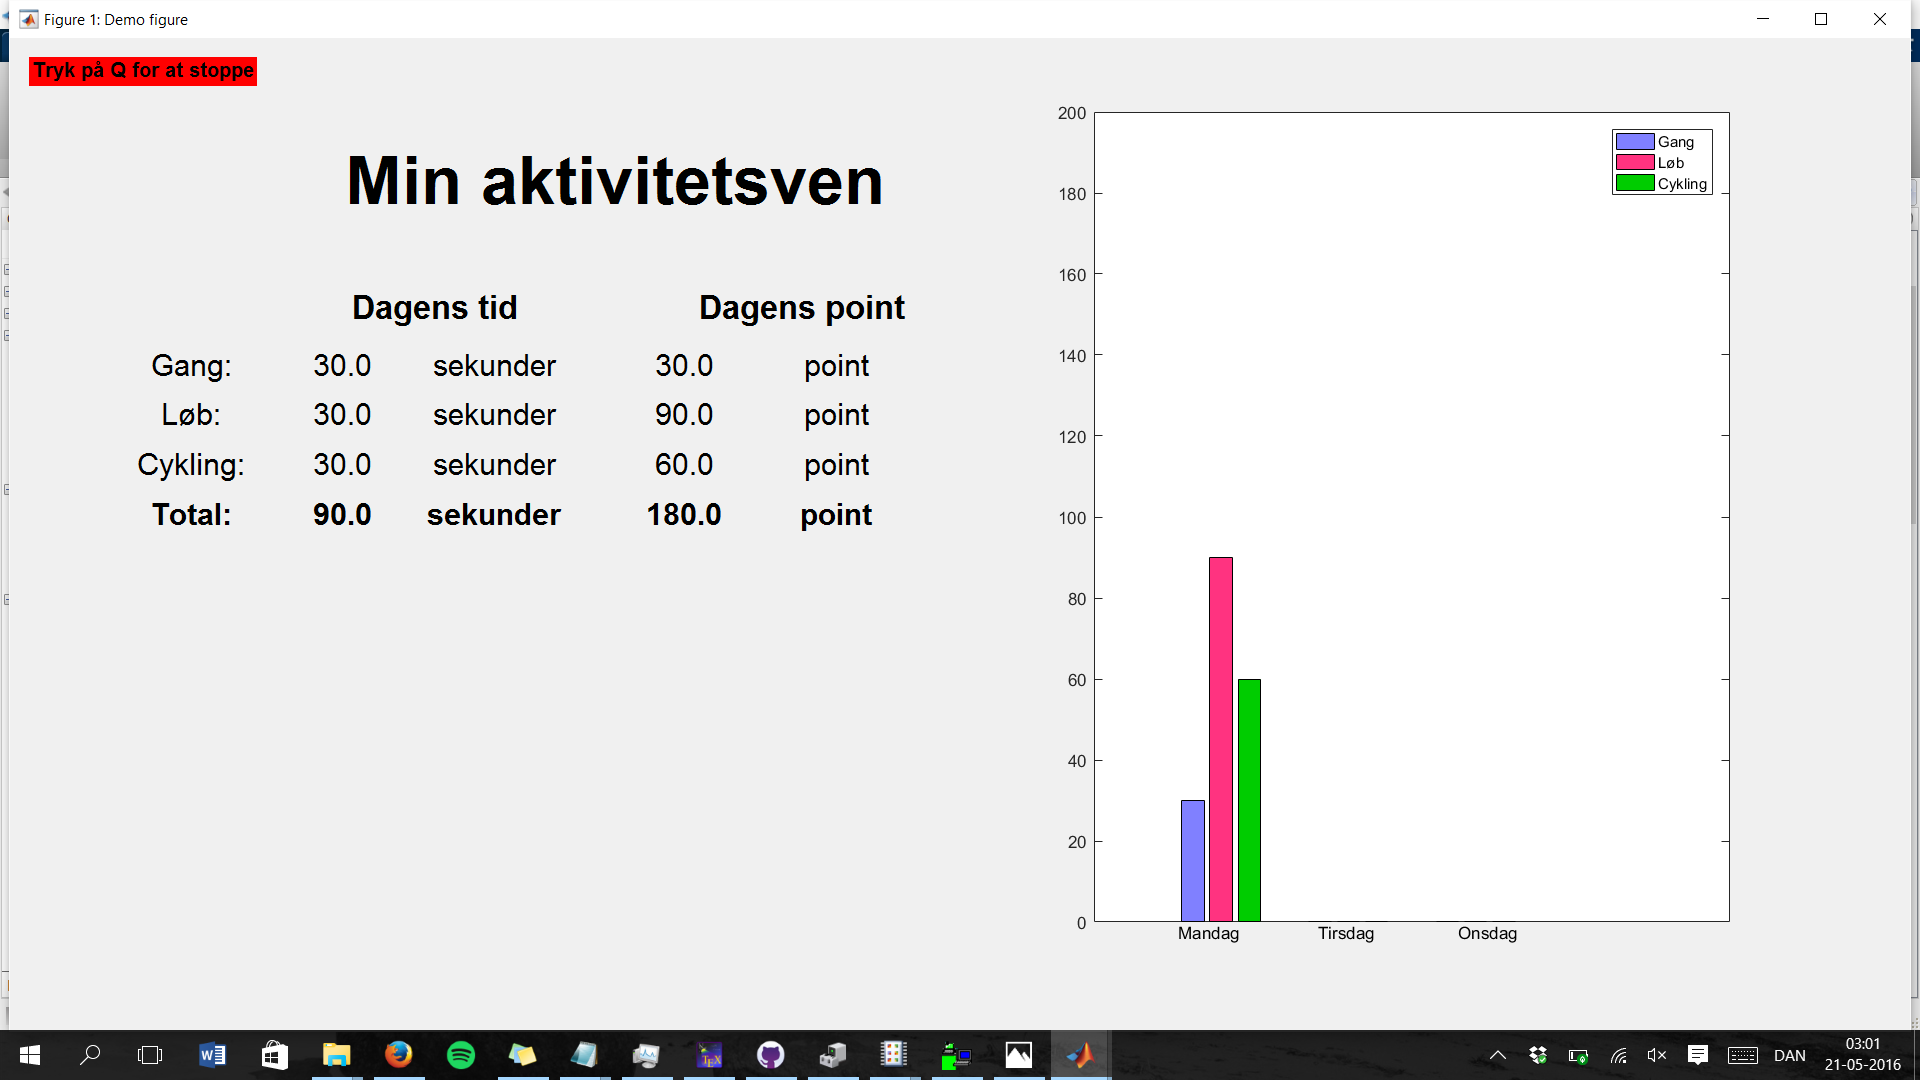
\includegraphics[scale=0.7]{figures/cDesign/test_GUI.png}
	\caption{På figuren ses et udklip af GUI hvor udførslen af aktiviteterne gang, løb og cykling visualiseres. Aktiviteternes samlede antal point og udført varighed ses på figuren.}
	\label{fig:GUI}
\end{figure}

Efterfulgt af design, implementering og test af GUI, kan det konkluderes at denne opfylder kravene heraf. GUI er i stand til at visualisere tidsforbruget samt antal point opnået, for alle aktiviteterne. GUI opdaterede kontinuert i testen hver gang et nyt input blev indsendt, hvoraf kravet vedrørende opdatering af GUI mindst hvert femtende minut, ligeledes er opfyldt.